% Chapter Template

\chapter{Results} % Main chapter title

\label{Chapter5} % Change X to a consecutive number; for referencing this chapter elsewhere, use \ref{ChapterX}

%----------------------------------------------------------------------------------------
%	SECTION 1
%----------------------------------------------------------------------------------------

\section{Balance Sheet Ratios}

The average observed liquidity ratios shown in Figure \ref{fig:Ratios} for all companies of the dataset are showing an increase in liquidity in 2020 and 2021 compared to the pre pandemic years indication that companies are holding relatively more cash at the year-end since the pandemic. A study conducted by the German Federal Bank reported an increase in the average cash ratio for German companies in 2020 as well as in 2021 \parencite{deutsche_bundesbank_jahresabschlussstatistik_2022}. For example, for SME corporations the study reported a change in the cash ratio from 0.104 (2019) to 0.110 (2020). For the current ratio and quick ratio, the same trend was reported. Further support for an increase in the quick ratio was found by another study \parencite{bley_mittelstand_2022}. Although the exact ratios are varying between studies, there is strong support for the general trend of increasing liquidity in 2020 and 2021.

Solvency ratios are showing a less clear trend after the COVID-19 pandemic. Although minimal, the opposite trends in the equity ratio and debt-to-asset-ratio are as expected. The only visible change happened in 2020, while in 2021 the ratios are very similar to 2018 and 2019. The change in the debt-to-asset ratio is amplified in the debt-to-equity ratio, as expected. Survy Data from the KFW found an Equity Ratio of 0.318 in 2019, a decrease to 0.301 in 2020 and a recovery to 0.314 in 2021 \parencite{kfw_kfw-mittelstandspanel_2022}. For very small companies with less than 10 employees, the drop in 2020 was stronger, and the recovery in 2021 was above pre-pandemic levels. Lager companies did not have a recovery after the crisis year and decreased their Equity Ratio in 2021 on average further. This could indicate that the recovery of the indebtedness in 2021 might have been driven by smaller companies. Similar observations were reported by the German Federal Bank were the debt-to-asset-ratio for SME corporations decreased in 2020.


\begin{figure}
\centering
\makebox[\textwidth][c]{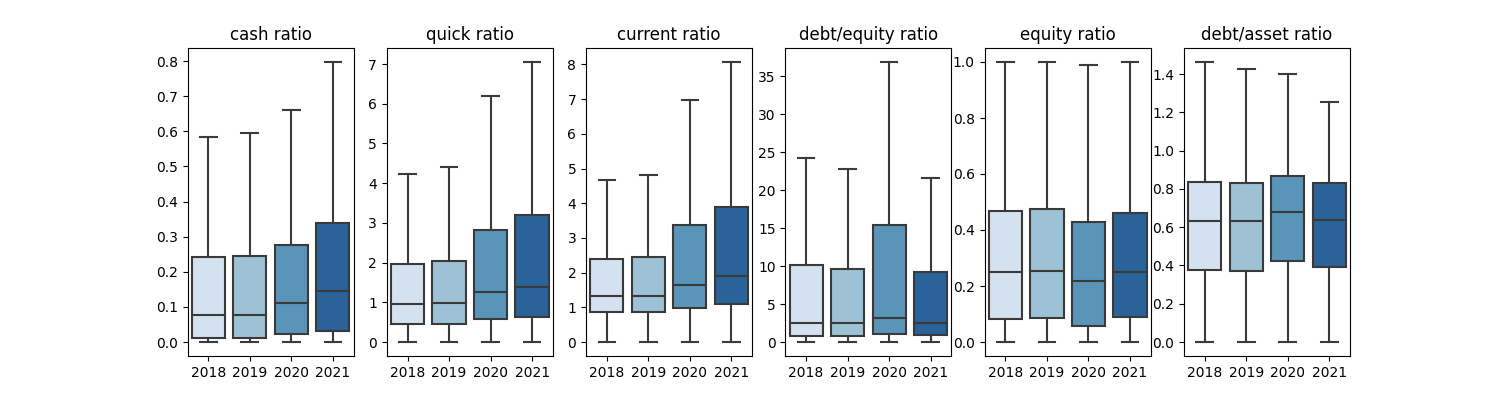
\includegraphics[width=1.2\columnwidth]{Figures/chart_ratios}}%

\decoRule
\caption[Balance sheet ratios]{Boxplot with balance sheet ratios from the obained dataset.}
\label{fig:Ratios}
\end{figure}


%----------------------------------------------------------------------------------------
%	SECTION 2
%----------------------------------------------------------------------------------------

\section{Diff and Diff}

\begin{table}
    \caption{Government aid impact on ratios}
    \label{tab:DiDresults}
    \centering
    \def\arraystretch{1.8}
    \centering
    \begin{tabular}{llrr}
\toprule
                     & \textbf{year} &                                    2020 &                                    2021 \\
{} & \textbf{instrument} &                                         &                                         \\
\midrule
\multirow{2}{*}{\textbf{cash ratio}} & \textbf{grant} &  -0.0089\space\space\space\space(0.270) &                  0.0768***\space(0.000) \\
                     & \textbf{loan} &                  0.0527***\space(0.000) &                  0.0351***\space(0.000) \\
\cline{1-4}
\multirow{2}{*}{\textbf{quick ratio}} & \textbf{grant} &  -0.0937\space\space\space\space(0.221) &   0.0913\space\space\space\space(0.478) \\
                     & \textbf{loan} &                  0.1085***\space(0.000) &   0.0929\space\space\space\space(0.252) \\
\cline{1-4}
\multirow{2}{*}{\textbf{current ratio}} & \textbf{grant} &  -0.0825\space\space\space\space(0.330) &   0.0476\space\space\space\space(0.736) \\
                     & \textbf{loan} &                  0.1271***\space(0.000) &        0.1828*\space\space\space(0.064) \\
\cline{1-4}
\multirow{2}{*}{\textbf{debt to equity ratio}} & \textbf{grant} &        0.2478*\space\space\space(0.089) &  -0.1592\space\space\space\space(0.185) \\
                     & \textbf{loan} &                  0.7306***\space(0.000) &             0.5043**\space\space(0.016) \\
\cline{1-4}
\multirow{2}{*}{\textbf{equity ratio}} & \textbf{grant} &  -0.0112\space\space\space\space(0.371) &   0.0108\space\space\space\space(0.465) \\
                     & \textbf{loan} &                 -0.0486***\space(0.000) &                  -0.037***\space(0.004) \\
\cline{1-4}
\multirow{2}{*}{\textbf{debt to assest ratio}} & \textbf{grant} &                  0.0412***\space(0.006) &       -0.0302*\space\space\space(0.079) \\
                     & \textbf{loan} &                  0.0715***\space(0.000) &                  0.0526***\space(0.002) \\
\bottomrule
\end{tabular}
}

    \small  Notes: Standard errors in parentheses, *** p<0.01, ** p<0.05, * p<0.1

    \end{table}
    
%----------------------------------------------------------------------------------------
%	SECTION 3
%----------------------------------------------------------------------------------------

\section{Causal Curve}

